As discussed in
Chapter~\ref{chapter:alternative_ssa_construction_algorithms}, loop
nesting forests complement the CFG and the dominance tree by
containing explicit information about the loops of an imperative
program, and in particular the way loops are nested inside each other.
The primary purpose of loop nesting forests is that of an auxiliary
intermediate data structure during the construction of SSA, for
efficient calculation of the iterated dominance frontier. However,
nesting forests may also themselves be represented in functional
languages.

Using the example from Figure~\ref{fig:lnf}, we outline possible
representations for reducible control-flow graphs, following the idea
that loops are explicitly modeled as a separate function declarations,
contained inside one another according to the loop nesting structure.

Our initial representation arises from the loop nesting forest from
Figure~\ref{fig:lnf}(b), if we interpret arcs as containment
relations between the declarations of functions $f_i$ that are fully
$\lambda$-lifted, i.e.~are equipped with their respective parameter
lists $\param i$ according to our initial liveness analysis. The given
forest yields code according to the following skeleton.
\begin{equation}
\label{FunctionalLoopNest1}
\begin{array}{l}
\mathtt{function}\ f_1(\param 1)\ = \\
  \quad
  \begin{array}{l}
     \mathtt{let}\ \ldots  \\
     \mathtt{in}\ 
     \begin{array}[t]{l}
       \mathtt{function}\ \loopfun_2 (\param 2) =  \\
       \quad \begin{array}[t]{l}
               \mathtt{function}\ f_2(\param 2) = \ldots \mathtt{in}\ \ite \ldots {f_3(\param 3)} {f_7(\param 7)}\\
               \mathtt{and}\ f_3(\param 3) = \ldots \mathtt{in}\ \ite \ldots {f_4(\param 4)} {f_5(\param 5)}\\
               \mathtt{and}\ f_4(\param 4) = \ldots \mathtt{in}\ f_6(\param 6)\\
               \mathtt{and}\ f_5(\param 5) = \ldots \mathtt{in}\ f_6(\param 6)\\
               \mathtt{and}\ f_6(\param 6) = \ldots \mathtt{in}\ f_8(\param 8)\\
               \mathtt{and}\ f_7(\param 7) = \ldots \mathtt{in}\ f_8(\param 8)\\
               \mathtt{and}\ f_8(\param 8) = \ldots \mathtt{in}\ \loopfun_9(\param 9)\\
               \mathtt{and}\ f_{12}(\param {12}) = \ldots \mathtt{in}\ \loopfun_2(\param 2)\\
               \mathtt{and}\ \loopfun_9 (\param 9) =  \\
                    \quad \begin{array}[t]{l}
                             \mathtt{function}\ f_9(\param 9) = \ldots \mathtt{in}\ \ite \ldots {f_{10}(\param {10})} {f_{11}(\param{11})}\\
                             \mathtt{and}\ f_{10}(\param {10}) = \ldots \mathtt{in}\ f_{11}(\param{11})\\
                             \mathtt{and}\ f_{11}(\param {11}) = \ldots \mathtt{in}\ \ite \ldots {\loopfun_9(\param 9)} {f_{12}(\param{12})}\\
                             \mathtt{in}\ f_9(\param 9)\ \mathtt{end}
                          \end{array}\\
               \mathtt{in}\ f_2(\param 2)\ \mathtt{end}
             \end{array}\\
       \mathtt{in}\ \loopfun_2(\param 2)\ \mathtt{end}
     \end{array}
  \end{array}\\ 
\mathtt{end}
\end{array} 
\end{equation}
In addition to functions $f_1, \ldots, f_{12}$ for the nodes of the
CFG, we introduce declarations for functions $\loopfun_2$ and
$\loopfun_9$. These model the loop header nodes drawn as ellipses in
Figure~\ref{fig:lnf}(b) and represent the outer and inner loop from
Figure~\ref{fig:lnf}(a), respectively.  The nodes constituting each
loop are organized as a single block of function declarations, in
accordance with the lack of more fine-grained structure in the loop
nesting forest in Figure~\ref{fig:lnf}(b). The loopback edges $12 \to
2$ and $11 \to 9$ in the CFG result in calls to $\loopfun _2$ and
$\loopfun_9$ in the bodies of $f_{12}$ and $f_{11}$, respectively.  As
desired, the fact that the loop with header 9 is nested inside the
loop with header 2 is explicitly captured: the declaration for
$\loopfun_9$ is nested inside the declaration for $\loopfun_2$.  As
$f_2$ is the unique header of the outer loop, the live-in variables of
$\loopfun_2$ are precisely $\param 2$; similarly, $\param 9$ are the
parameters of $\loopfun_9$.

Code~(\ref{FunctionalLoopNest1}) may be improved in two respects. The
first optimization combines the nesting information between loops with
dominance information within loops and thus refines the structure of
each loop's block of function declarations.
Figure~\ref{FigureCFGForLoopNestFromChapter4} depicts on the left the
CFG obtained from Figure~\ref{fig:lnf}(a) by adding explicit nodes
$\loopfun_2$ and $\loopfun_9$, and on the right the corresponding
dominance tree.
\begin{figure}
\begin{center}
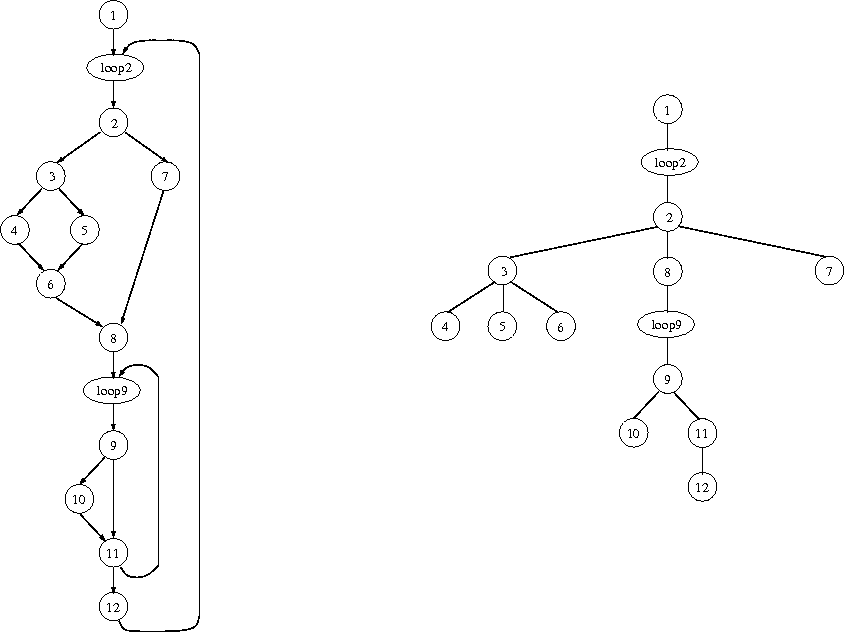
\includegraphics[scale=0.4]{LoopNestingCFG}
\end{center}
\caption{\label{FigureCFGForLoopNestFromChapter4} (a) control-flow graph from Figure~\ref{fig:lnf}, extended by loop nesting nodes. (b) Dominance graph}
\end{figure} As before, we may interpret
this mixed loop nesting/dominance tree as specification for the
application of block sinking -- see the code in
Figure~\ref{fig:part1:sematics:FunctionalLoopNest2}.

\begin{equation}
\label{FunctionalLoopNest2}
%\begin{figure}
%$$
\begin{array}{l}
\mathtt{function}\ f_1(\param 1)\ = \\
  \quad
  \begin{array}{l}
     \mathtt{let}\ \ldots  \\
     \mathtt{in}\ 
     \begin{array}[t]{l}
       \mathtt{function}\ \loopfun_2 (\param 2) =  \\
       \quad \begin{array}[t]{l}
               \mathtt{function}\ f_2(\param 2) = \\
               \quad \mathtt{let} \ldots \textit{(* let-bindings of $f_2$ *)} \ldots\\
               \quad \mathtt{in}\ 
                       \begin{array}[t]{l} 
                         \mathtt{function}\ f_3(\param 3) = \\
                         \quad \mathtt{let} \ldots \textit{(* let-bindings of $f_3$ *)} \ldots\\
                         \quad \mathtt{in}\ 
                               \begin{array}[t]{l}
                                 \mathtt{function}\ f_4(\param 4) = \ldots \mathtt{in}\ f_6(\param 6)\\
                                 \mathtt{and}\ f_5(\param 5) = \ldots \mathtt{in}\ f_6(\param 6)\\
                                 \mathtt{and}\ f_6(\param 6) = \ldots \mathtt{in}\ f_8(\param 8)\\
                                 \mathtt{in}\ \ite \ldots {f_4(\param 4)} {f_5(\param 5)}\ \mathtt{end}
                               \end{array}\\
                         \quad \mathtt{end}\ \textit{(* of $f_3$'s declaration *)}\\
                         \mathtt{and}\ f_7(\param 7) = \ldots \mathtt{in}\ f_8(\param 8)\\
                         \mathtt{and}\ f_8(\param 8) = \\
                         \quad \mathtt{let} \ldots \textit{(* let-bindings of $f_8$ *)} \ldots\\
                         \quad \mathtt{in}\ 
                               \begin{array}[t]{l}
                                  \mathtt{function}\ \loopfun_9 (\param 9) =  \\
                                  \quad \begin{array}[t]{l}
                                       \mathtt{function}\ f_9(\param 9) = \\
                                       \quad \mathtt{let} \ldots \textit{(* let-bindings of $f_9$ *)} \ldots\\
                                       \quad \mathtt{in}\ 
                                             \begin{array}[t]{l}
                                                \mathtt{function}\ f_{10}(\param {10}) = \ldots 
                                                                  \mathtt{in}\ f_{11}(\param{11})\\
                                                \mathtt{and}\ f_{11}(\param {11}) = \\
                                                     \quad \mathtt{let} \ldots \textit{(* let-bindings of $f_{11}$ *)} \ldots\\
                                                     \quad \mathtt{in}\ 
                                                           \begin{array}[t]{l}
                                                              \mathtt{function}\ f_{12}(\param {12}) = 
                                                                                \ldots \mathtt{in}\ \loopfun_2(\param 2)\\
                                                              \mathtt{in}\ \ite \ldots {\loopfun_9(\param 9)} 
                                                                                    {f_{12}(\param{12})}\
                                                              \mathtt{end}
                                                           \end{array}\\
                                                      \quad \mathtt{end}\ \textit{(* of $f_{11}$'s declaration *)}\\
                                                \mathtt{in}\ \ite \ldots {f_{10}(\param {10})}
                                                                         {f_{11}(\param{11})}\ 
                                                             \mathtt{end}
                                             \end{array}\\
                                       \quad \mathtt{end}\ \textit{(* of $f_9$'s\ declaration *)}\\
                             \mathtt{in}\ f_9(\param 9)\ \mathtt{end}\ \textit{(* of\ $\loopfun_9$'s\ declaration *)}
                          \end{array}\\
                                 \mathtt{in}\ \loopfun_9(\param 9)\ \mathtt{end} 
                               \end{array}\\
                         \quad \mathtt{end}\ \textit{(* of $f_8$'s declaration *)}\\
                         \mathtt{in}\ \ite \ldots {f_3(\param 3)} {f_7(\param 7)}\ \mathtt{end}
                       \end{array} \\
               \quad \mathtt{end}\ \textit{(* of $f_2$'s declaration *)}\\      
               \mathtt{in}\ f_2(\param 2)\ \mathtt{end}\ \textit{(* of\ $\loopfun_2$'s\ declaration *)}
             \end{array}\\
       \mathtt{in}\ \loopfun_2(\param 2)\ \mathtt{end}
     \end{array}
  \end{array}\\ 
\mathtt{end}\ \textit{(*of\ $f_1$'s\ declaration*)}
\end{array} 
%$$
%\caption{\label{fig:part1:sematics:FunctionalLoopNest2}
%   Functional representation according to the nesting suggested 
%    by the graph in Figure~\ref{FigureCFGForLoopNestFromChapter4}.}
%\end{figure}
\end{equation}

The most interesting aspect of the mixed graph (and of
code~(\ref{FunctionalLoopNest2})) is the position of node $12$. In
contrast to Figure~\ref{fig:lnf}(b), where $12$ is an immediate child
of $\loopfun_2$, we have given precedence to the dominance relation,
which suggests insertion underneath node $11$: while node $12$ not a
\emph{constituent} of the loop $9-10-11$, it
\emph{is dominated} by this loop. We are unaware of discussions or
formal definitions of such mixed loop-nesting/dominance graphs in the
literature, but remark that the chosen insertion policy again brings
the declaration of $f_{12}$ closer to its call sites, increasing the
potential to drop parameters from $f_{12}$, namely all parameters
whose arguments are supplied in the bodies of $f_2$, $f_8$, $f_9$, and
$f_{11}$.  Nevertheless, inserting the declaration of $f_{12}$ in
parallel to that of $f_2$, immediately inside the definition of
$\loopfun_2$, would be equally sound from a functional perspective,
and so would be the insertion of $f_{12}$ anywhere along the path
$\loopfun_2 \to 2 \to 8 \to \loopfun_9 \to 9 \to 11$ in the mixed
graph.

The second optimization modifies the call structure by changing the
target nodes of the loopback edges. Instead of inserting recursive calls to
$\loopfun_2$ and $\loopfun_9$ as in code~(\ref{FunctionalLoopNest1}),
we insert calls to $f_2$ and $f_9$, as highlighted in
code~(\ref{FunctionalLoopNest3}):
\begin{equation}
\label{FunctionalLoopNest3}
\begin{array}{l}
\mathtt{function}\ f_1(\param 1)\ = \\
  \quad
  \begin{array}{l}
     \mathtt{let}\ \ldots  \\
     \mathtt{in}\ 
     \begin{array}[t]{l}
       \mathtt{function}\ \loopfun_2 (\param 2) =  \\
       \quad \begin{array}[t]{l}
               \mathtt{function}\ f_2(\param 2) = \ldots \mathtt{in}\ \ite \ldots {f_3(\param 3)} {f_7(\param 7)}\\
               \mathtt{and}\ f_3(\param 3) = \ldots \mathtt{in}\ \ite \ldots {f_4(\param 4)} {f_5(\param 5)}\\
               \mathtt{and}\ f_4(\param 4) = \ldots \mathtt{in}\ f_6(\param 6)\\
               \mathtt{and}\ f_5(\param 5) = \ldots \mathtt{in}\ f_6(\param 6)\\
               \mathtt{and}\ f_6(\param 6) = \ldots \mathtt{in}\ f_8(\param 8)\\
               \mathtt{and}\ f_7(\param 7) = \ldots \mathtt{in}\ f_8(\param 8)\\
               \mathtt{and}\ f_8(\param 8) = \ldots \mathtt{in}\ f_9(\param 9)\\
               \mathtt{and}\ f_{12}(\param {12}) = \ldots \mathtt{in}\ \fbox{$f_2(\param 2)$}\\
               \mathtt{and}\ \loopfun_9 (\param 9) =  \\
                    \quad \begin{array}[t]{l}
                             \mathtt{function}\ f_9(\param 9) = \ldots \mathtt{in}\ \ite \ldots {f_{10}(\param {10})} {f_{11}(\param{11})}\\
                             \mathtt{and}\ f_{10}(\param {10}) = \ldots \mathtt{in}\ f_{11}(\param{11})\\
                             \mathtt{and}\ f_{11}(\param {11}) = \ldots \mathtt{in}\ \ite \ldots {\fbox{$f_9(\param 9)$}} {f_{12}(\param{12})}\\
                             \mathtt{in}\ \loopfun_9(\param 9)\ \mathtt{end}
                          \end{array}\\
               \mathtt{in}\ f_2(\param 2)\ \mathtt{end}
             \end{array}\\
       \mathtt{in}\ \loopfun_2(\param 2)\ \mathtt{end}
     \end{array}
  \end{array}\\ 
\mathtt{end}
\end{array} 
\end{equation}
This modification reduces the number of function calls per loop
iteration by one. Effectively, the explicit loop \emph{header} nodes
$\loopfun_2$ and $\loopfun_9$ are turned into loop \emph{pre}headers
which may, for example, be used for placing instructions that are
hoisted from the respective loops but cannot be inserted into the loop
predecessors.

The two optimizations are independent from each other and can be
applied in either order. In particular, adding nodes for $\loopfun_2$
and $\loopfun_9$ according to the call structure of
(\ref{FunctionalLoopNest3}) into the CFG from Figure~\ref{fig:lnf}(a)
and again calculating the dominance tree yields the same mixed loop
nest/dominance graph as given in
Figure~\ref{FigureCFGForLoopNestFromChapter4}(b). Thus, applying block
sinking to code~(\ref{FunctionalLoopNest3}) yields code with the
nesting structure of~(\ref{FunctionalLoopNest2}) but the call structure
of~(\ref{FunctionalLoopNest3}). Alternatively, we may obtain this code
by altering the loopback calls in the bodies of $f_{12}$ and $f_{11}$
of~(\ref{FunctionalLoopNest2}) to target directly the functions $f_2$
and $f_9$, respectively, instead of $\loopfun_2$ and $\loopfun_9$.

All loop nesting formats discussed can subsequently be subjected to
parameter dropping as described in the previous sections. In the case
of loopback edges in the style of~(\ref{FunctionalLoopNest3}) it is in
fact possible to drop
\emph{all} parameters of $\loopfun_2$ and $\loopfun_9$: the only
calls to these functions directly follow their respective declarations
and are hence in the scope of the same bindings, so the conditions for
parameter dropping from
Section~\ref{section:Part1:Semantics:lambdaDropping:parameterDropping}
apply trivially.  In case of loopback edges according
to~(\ref{FunctionalLoopNest1}) and ~(\ref{FunctionalLoopNest2}), a
similar reasoning shows that all parameters $\param 2$ may be dropped
from $f_2$, and similarly $\param 9$ from $f_9$.

Finally, let us consider the variable of interest from
Figure~\ref{fig:lnf}, $v$, explicitly.  Extending
code~(\ref{FunctionalLoopNest2}) by appropriately indicating the three
definitions and the single use of $v$ yields
code~(\ref{FunctionalLoopNest2v}), under the simplifying assumption
that no other variables are present.
\begin{equation}
\label{FunctionalLoopNest2v}
\begin{array}{l}
\mathtt{function}\ f_1()\ = \\
  \quad
  \begin{array}{l}
     \mathtt{let}\ \ldots  \\
     \mathtt{in}\ 
     \begin{array}[t]{l}
       \mathtt{function}\ \loopfun_2 () =  \\
       \quad \begin{array}[t]{l}
               \mathtt{function}\ f_2() = \\
               \quad \mathtt{let} \ldots \textit{(* let-bindings of $f_2$ *)} \ldots\\
               \quad \mathtt{in}\ 
                       \begin{array}[t]{l} 
                         \mathtt{function}\ f_3() = \\
                         \quad \mathtt{let} \ldots \textit{(* let-bindings of $f_3$ *)} \ldots\\
                         \quad \mathtt{in}\ 
                               \begin{array}[t]{l}
                                 \mathtt{function}\ f_4() = \fbox{$\letin v \ldots {\ldots f_6(v)}$}\\
                                 \mathtt{and}\ f_5() = \fbox{$\letin v \ldots {\ldots f_6(v)}$}\\
                                 \mathtt{and}\ f_6(v) = \ldots \mathtt{in}\ f_8(v)\\
                                 \mathtt{in}\ \ite \ldots {f_4()} {f_5()}\ \mathtt{end}
                               \end{array}\\
                         \quad \mathtt{end}\ \textit{(* of $f_3$'s declaration *)}\\
                         \mathtt{and}\ f_7() = \fbox{$\letin v \ldots {\ldots f_8(v)}$}\\
                         \mathtt{and}\ f_8(v) = \\
                         \quad \mathtt{let} \ldots \textit{(* let-bindings of $f_8$ *)} \ldots\\
                         \quad \mathtt{in}\ 
                               \begin{array}[t]{l}
                                  \mathtt{function}\ \loopfun_9 (v) =  \\
                                  \quad \begin{array}[t]{l}
                                       \mathtt{function}\ f_9(v) = \\
                                       \quad \fbox{$\mathtt{let}\ \ldots = v \ldots$}\\
                                       \quad \mathtt{in}\ 
                                             \begin{array}[t]{l}
                                                \mathtt{function}\ f_{10}(v) = \ldots 
                                                                  \mathtt{in}\ f_{11}(v)\\
                                                \mathtt{and}\ f_{11}(v) = \\
                                                     \quad \mathtt{let} \ldots \textit{(* let-bindings of $f_{11}$ *)} \ldots\\
                                                     \quad \mathtt{in}\ 
                                                           \begin{array}[t]{l}
                                                              \mathtt{function}\ f_{12}() = 
                                                                 \fbox{$\letin v \ldots {\ldots \loopfun_2()}$}\\
                                                              \mathtt{in}\ \ite \ldots {\loopfun_9(v)} 
                                                                                    {f_{12}()}\
                                                              \mathtt{end}
                                                           \end{array}\\
                                                      \quad \mathtt{end}\ \textit{(* of $f_{11}$'s declaration *)}\\
                                                \mathtt{in}\ \ite \ldots {f_{10}(v)}
                                                                         {f_{11}(v)}\ 
                                                             \mathtt{end}
                                             \end{array}\\
                                       \quad \mathtt{end}\ \textit{(* of $f_9$'s\ declaration *)}\\
                             \mathtt{in}\ f_9(v)\ \mathtt{end}\ \textit{(* of\ $\loopfun_9$'s\ declaration *)}
                          \end{array}\\
                                 \mathtt{in}\ \loopfun_9(v)\ \mathtt{end} 
                               \end{array}\\
                         \quad \mathtt{end}\ \textit{(* of $f_8$'s declaration *)}\\
                         \mathtt{in}\ \ite \ldots {f_3()} {f_7()}\ \mathtt{end}
                       \end{array} \\
               \quad \mathtt{end}\ \textit{(* of $f_2$'s declaration *)}\\      
               \mathtt{in}\ f_2()\ \mathtt{end}\ \textit{(* of\ $\loopfun_2$'s\ declaration *)}
             \end{array}\\
       \mathtt{in}\ \loopfun_2()\ \mathtt{end}
     \end{array}
  \end{array}\\ 
\mathtt{end}\ \textit{(*of\ $f_1$'s\ declaration*)}
\end{array} 
\end{equation}
In particular, the initial liveness analysis yields $\{v\} = \param 9
= \param {11} = \param {10} = \param {8} = \param {6}$, and $\param i
= \emptyset$ for $i \notin \{9,11,10,8,6\}$.  The conditions for
parameter dropping outlined in
Section~\ref{section:Part1:Semantics:lambdaDropping:parameterDropping}
sanction the removal of $v$ from the declarations of (in this order)
$f_{10}/f_{11}$, $f_9$, and $\loopfun_9$, since all uses of $v$ in the
loop $9-10-11$ are bound by the formal parameter of $f_8$.  Thus, only
the occurrences of $v$ in the parameter lists of $f_6$ and $f_8$
remain, in accordance with the minimality condition from
Section~\ref{sec:properties_and_flavors:minimality}: the join points
for the definition set $X=\{4, 5, 7\}$ are precisely nodes $6$ and
$8$. The difference to the outcome of the algorithm for computing the
iterated dominance frontier from
Section~\ref{section:alternative_ssa_construction_algorithms:loop} is
explained by our initial use of liveness information, which eliminates
node $12$ from the set $X$ of relevant def-sites. We expect that a
modification of the IDF algorithm that takes liveness information into
account would avoid the generation of a $\phi$-function for $v$ in
block $2$, and would yield pruned SSA in general. A structural
difference between our approach and the algorithm from
Section~\ref{section:alternative_ssa_construction_algorithms:loop} is
that our discussion
\emph{assumes} dominance information when applying block sinking
whereas the IDF algorithm implicitly \emph{calculates} such
information, separately for each variable under
consideration\footnote{There's probably a version of the algorithm
that does the job for all variables in one go. Is it described in the
book?}.


% \subsection{To be removed}
% In the functional setting, this discipline
% amounts to a small modification of block-sinking: functions $f$ that
% are called from within a \emph{recursive} function $g$ are placed at
% the \emph{same} level as $g$ rather than \emph{inside} $g$. Returning
% to our running example, we place $f_3$ at the same level as $f_2$, in
% contrast to code~(\ref{FunctionalConstructionProgram4}).  The
% placement of both functions relative to $f_1$ is left unaltered.

% \begin{equation}
% \label{FunctionalConstructionProgram7}
% \begin{array}{l}
% \mathtt{function}\ f_1()\ = \\
%   \quad
%   \begin{array}{l}
%      \mathtt{let}\ v = 1 \ 
%      \mathtt{in\ let}\ z = 8 \ 
%      \mathtt{in\ let}\ y = 4\\
%      \mathtt{in}\ 
%      \begin{array}[t]{l}
%        \mathtt{function}\ f_3(y,v) = 
%           \mathtt{let}\ w = y+v\ \mathtt{in}\ w\ \mathtt{end}\\
%        \mathtt{and}\ f_2(v,z,y) =\\
%          \quad
%          \begin{array}{l}
%            \mathtt{let}\ x = 5+y\
%            \mathtt{in\ let}\ y = x*z\
%            \mathtt{in\ let}\ x = x-1\\
%            \mathtt{in}\
%              \mathtt{if}\ x=0\
%              \mathtt{then}\ f_3(y,v)\ 
%              \mathtt{else}\ f_2(v,z,y)\\
%            \mathtt{end\ end\ end}
%          \end{array}\\
%      \mathtt{in}\ f_2(v,z,y)\ \mathtt{end}
%      \end{array}\\
%      \mathtt{end\ end\ end}\\
%    \end{array}\\
% \mathtt{in}\ f_1()\  \mathtt{end}
% \end{array}
% \end{equation}
% As a consequence, any parameter of $f$ that is rebound in $g$ cannot
% be dropped. In the example, $y$ is not deleted from the parameter list
% of $f_3$, as the declaration of $f_3$ is not any longer in the scope
% of the binding for $y$ that applies at the call to $f_3$. In contrast,
% $v$ may still be dropped from $f_3$, and $v$ and $z$ may be dropped
% from $f_2$:
% \begin{equation}
% \label{FunctionalConstructionProgram8}
% \begin{array}{l}
% \mathtt{function}\ f_1()\ = \\
%   \quad
%   \begin{array}{l}
%      \mathtt{let}\ v = 1 \ 
%      \mathtt{in\ let}\ z = 8 \ 
%      \mathtt{in\ let}\ y = 4\\
%      \mathtt{in}\ 
%      \begin{array}[t]{l}
%        \mathtt{function}\ f_3(y) = 
%           \mathtt{let}\ w = y+v\ \mathtt{in}\ w\ \mathtt{end}\\
%        \mathtt{and}\ f_2(y) =\\
%          \quad
%          \begin{array}{l}
%            \mathtt{let}\ x = 5+y\
%            \mathtt{in\ let}\ y = x*z\
%            \mathtt{in\ let}\ x = x-1\\
%            \mathtt{in}\
%              \mathtt{if}\ x=0\
%              \mathtt{then}\ f_3(y)\ 
%              \mathtt{else}\ f_2(y)\\
%            \mathtt{end\ end\ end}
%          \end{array}\\
%      \mathtt{in}\ f_2(y)\ \mathtt{end}
%      \end{array}\\
%      \mathtt{end\ end\ end}\\
%    \end{array}\\
% \mathtt{in}\ f_1()\  \mathtt{end}
% \end{array}
% \end{equation}
% If we unroll $f_2$ in this loop-closed form and replace the recursive
% call to $f_2$ by a call to its copy $f_{2'}$ we obtain
% code~(\ref{FunctionalConstructionProgramUnrolled}).
% \begin{equation}
% \label{FunctionalConstructionProgramUnrolled}
% \begin{array}{l}
% \mathtt{function}\ f_1()\ = \\
%   \quad
%   \begin{array}{l}
%      \mathtt{let}\ v = 1 \ 
%      \mathtt{in\ let}\ z = 8 \ 
%      \mathtt{in\ let}\ y = 4\\
%      \mathtt{in}\ 
%      \begin{array}[t]{l}
%        \mathtt{function}\ f_3(y) = 
%           \mathtt{let}\ w = y+v\ \mathtt{in}\ w\ \mathtt{end}\\
%        \mathtt{and}\ f_2(y) =\\
%          \quad
%          \begin{array}{l}
%            \mathtt{let}\ x = 5+y\
%            \mathtt{in\ let}\ y = x*z\
%            \mathtt{in\ let}\ x = x-1\\
%            \mathtt{in}\
%            \begin{array}[t]{l}
%              \mathtt{if}\ x=0\\
%              \mathtt{then}\ f_3(y)\\ 
%              \mathtt{else}\
%                \begin{array}[t]{l}
%                  \mathtt{function}\ f_{2'}(y) =\\
%                  \quad
%                  \begin{array}{l}
%                    \mathtt{let}\ x = 5+y\
%                    \mathtt{in\ let}\ y = x*z\
%                    \mathtt{in\ let}\ x = x-1\\
%                    \mathtt{in}\
%                      \mathtt{if}\ x=0\
%                      \mathtt{then}\ f_3(y)\ 
%                      \mathtt{else}\ f_2(y)\\
%                    \mathtt{end\ end\ end}
%                  \end{array}\\
%                  \mathtt{in}\ f_{2'}(y)\ \mathtt{and}
%                \end{array}
%            \end{array}\\
%            \mathtt{end\ end\ end}
%          \end{array}\\
%      \mathtt{in}\ f_2(y)\ \mathtt{end}
%      \end{array}\\
%      \mathtt{end\ end\ end}\\
%    \end{array}\\
% \mathtt{in}\ f_1()\  \mathtt{end}
% \end{array}
% \end{equation}
% Having nested $f_{2'}$ inside $f_2$, we may immediately drop parameter
% $y$ from $f_{2'}$, yielding
% code~(\ref{FunctionalConstructionProgram9}).
% \begin{equation}
% \label{FunctionalConstructionProgram9}
% \begin{array}{l}
% \mathtt{function}\ f_1()\ = \\
%   \quad
%   \begin{array}{l}
%      \mathtt{let}\ v = 1 \ 
%      \mathtt{in\ let}\ z = 8 \ 
%      \mathtt{in\ let}\ y = 4\\
%      \mathtt{in}\ 
%      \begin{array}[t]{l}
%        \mathtt{function}\ f_3(y) = 
%           \mathtt{let}\ w = y+v\ \mathtt{in}\ w\ \mathtt{end}\\
%        \mathtt{and}\ f_2(y) =\\
%          \quad
%          \begin{array}{l}
%            \mathtt{let}\ x = 5+y\
%            \mathtt{in\ let}\ y = x*z\
%            \mathtt{in\ let}\ x = x-1\\
%            \mathtt{in}\
%            \begin{array}[t]{l}
%              \mathtt{if}\ x=0\\
%              \mathtt{then}\ f_3(y)\\ 
%              \mathtt{else}\
%                \begin{array}[t]{l}
%                  \mathtt{function}\ f_{2'}() =\\
%                  \quad
%                  \begin{array}{l}
%                    \mathtt{let}\ x = 5+y\
%                    \mathtt{in\ let}\ y = x*z\
%                    \mathtt{in\ let}\ x = x-1\\
%                    \mathtt{in}\
%                      \mathtt{if}\ x=0\
%                      \mathtt{then}\ f_3(y)\ 
%                      \mathtt{else}\ f_2(y)\\
%                    \mathtt{end\ end\ end}
%                  \end{array}\\
%                  \mathtt{in}\ f_{2'}()\ \mathtt{and}
%                \end{array}
%            \end{array}\\
%            \mathtt{end\ end\ end}
%          \end{array}\\
%      \mathtt{in}\ f_2(y)\ \mathtt{end}
%      \end{array}\\
%      \mathtt{end\ end\ end}\\
%    \end{array}\\
% \mathtt{in}\ f_1()\  \mathtt{end}
% \end{array}
% \end{equation}
% This code exhibits the same sharing as the loop-unrolled SSA program
% shown at the top of
% Figure~\ref{fig:FunctionalCorrespondenceSSAofLoopClosedProgram}.
% \begin{figure}
% \begin{center}
% 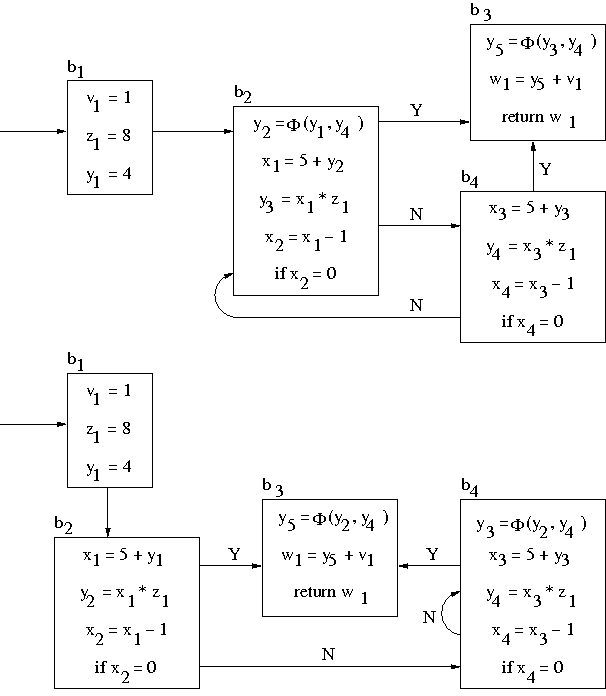
\includegraphics[scale=0.4]{SSAConstructionExample4}
% \end{center}
% \caption{\label{fig:FunctionalCorrespondenceSSAofLoopClosedProgram} Two outcomes of loop-unrolling, corresponding to programs~(\ref{FunctionalConstructionProgram9}) and~(\ref{FunctionalConstructionProgram10})}
% \end{figure}
% The invocations sites to $f_3$ correspond to the control-flow arcs
% with target $b_3$, each passing the appropriate value to the ``loop
% closing'' parameter $y$ of $f_3$.

% Note that when unrolling the loop, the call to $f_2$ inside the body
% of $f_{2'}$ was \emph{not} replaced by a call to $f_{2'}$. Indeed,
% performing this replacement would have amounted to peeling the first
% iteration off the loop, which - after parameter-dropping the $y$ now
% from the declaration of $f_2$ - would have yielded
% code~(\ref{FunctionalConstructionProgram10}) and the imperative code
% shown in the lower half of
% Figure~\ref{fig:FunctionalCorrespondenceSSAofLoopClosedProgram}.

% %The lower half of
% %Figure~\ref{fig:FunctionalCorrespondenceSSAofLoopClosedProgram} shows
% %an alternative outcome of loop unrolling. Here, the resulting loop
% %encompasses only $b_{2'}$. We obtain corresponding functional code if --
% %starting again from (\ref{FunctionalConstructionProgram8}) -- we first
% %place the initial copy of $f_2$ (again named $f_{2'}$) at the same
% %nesting level as $f_2$ and replace the call to $f_2$ inside $f_{2'}$ by a
% %recursive call to $f_{2'}$. The only invocation of $f_2$ that remains is
% %that in $f_1$, whereas two invocation sites exist for $f_{2'}$. We then
% %perform $\lambda$-dropping, which moves the definition $f_{2'}$ inside
% %that of $f_2$ and also drops the parameter $y$ from the declaration of
% %$f_2$:
% \begin{equation}
% \label{FunctionalConstructionProgram10}
% \begin{array}{l}
% \mathtt{function}\ f_1()\ = \\
%   \quad
%   \begin{array}{l}
%      \mathtt{let}\ v = 1 \ 
%      \mathtt{in\ let}\ z = 8 \ 
%      \mathtt{in\ let}\ y = 4\\
%      \mathtt{in}\ 
%      \begin{array}[t]{l}
%        \mathtt{function}\ f_3(y) = 
%           \mathtt{let}\ w = y+v\ \mathtt{in}\ w\ \mathtt{end}\\
%        \mathtt{and}\ f_2() =\\
%          \quad
%          \begin{array}{l}
%            \mathtt{let}\ x = 5+y\
%            \mathtt{in\ let}\ y = x*z\
%            \mathtt{in\ let}\ x = x-1\\
%            \mathtt{in}\
%            \begin{array}[t]{l}
%              \mathtt{if}\ x=0\\
%              \mathtt{then}\ f_3(y)\\ 
%              \mathtt{else}\
%                \begin{array}[t]{l}
%                  \mathtt{function}\ f_{2'}(y) =\\
%                  \quad
%                  \begin{array}{l}
%                    \mathtt{let}\ x = 5+y\
%                    \mathtt{in\ let}\ y = x*z\
%                    \mathtt{in\ let}\ x = x-1\\
%                    \mathtt{in}\
%                      \mathtt{if}\ x=0\
%                      \mathtt{then}\ f_3(y)\ 
%                      \mathtt{else}\ f_{2'}(y)\\
%                    \mathtt{end\ end\ end}
%                  \end{array}\\
%                  \mathtt{in}\ f_{2'}()\ \mathtt{and}
%                \end{array}
%            \end{array}\\
%            \mathtt{end\ end\ end}
%          \end{array}\\
%      \mathtt{in}\ f_2()\ \mathtt{end}
%      \end{array}\\
%      \mathtt{end\ end\ end}\\
%    \end{array}\\
% \mathtt{in}\ f_1()\  \mathtt{end}
% \end{array}
% \end{equation}
